\documentclass[]{article}


\usepackage{apacite}            % APA citation style 
\bibliographystyle{apacite} 
\usepackage{listings}           % for writing cod eparagraphs
\usepackage{graphicx}           % for adding figures
\usepackage{float}              % for fixing the table


% Manuscript header
\title{An R Package and a Shiny Application for Normative Analysis of Trail Making Test}

\author{
	E. F. Haghish %\\ Nicole von Steinbuchel 
}

\begin{document}

\maketitle

\begin{abstract}
	The Trail Making Test (TMT) is one of the common neuropsychological tests. The test measures performance time for two visual-conceptual and visual-motor tracking tasks. Knowing that different factors such as age, level of education, and general intelligence influence the TMT test, different norms and cut-off values have been published for interpreting the results. The current manuscript reviews some of the frequently used norms and cut-off values and introduces a software and an R package for interpreting the TMT performance time based on these norms.  
\end{abstract}

\section{Introduction}
	The Trail Making Test (TMT) was introduces within the Army Individual Test Battery in 1944 \cite{reitan1985halstead}. Due to the simplicity of administration and its sensitivity to brain damage \cite{reitan1955relation}, TMT has become one of the most popular neuropsychology tests. 
	
	TMT is a paper-and-pencil test, which includes two separate sections, part A and part B and is claimed to examine different cognitive constructs. The part A is concerned with attention \cite{seo2006} and requires the participants to connect numbered circles in ascending order. The circles are numbered from one to twenty-five and are randomly scattered over a paper. Part B is more related to executive function \cite{ble2005, seo2006} and is considered to be more difficult to perform, although there is no general agreement on the underlying cognitive constructs assessed by part B \cite{kortte2002}. Part B is consisted of two types of circles, numbered circles (from 1 to 12) and circles with alphabet letters (from A to L). In ascending order, the participants should connect each alphabetical letter to a number corresponding to its rank. For example, beginning with 1-A, 2-B, ..., and ending with 12-L. The time needed by a participant to finish each part correctly is recorded as a measurement of performance. 
	
	
	•	How the results of the test are interpreted?\\
	•	What are we doing in this manuscript\\
	o	What is wrong with the previous norms?\\
	

% THE NORMATIVE DATA
% ==================
\section{The normative data}
	
	
	
	
	
	
	
\section{\texttt{tmt} R package}

The main idea of the \texttt{tmt} R package was to develop a comprehensive pakage for normative transformation of the TMT scores. In contrast to applying a threshold for categorizing subjects as pathological or non-pathological based on TMT raw scores, the normative transformation allows to obtain a better understanding of the subject performance relative to his peers. 


\subsection{Installation}

The \texttt{tmt} package is hosted on CRAN and can be installed directly from within R as follows.

\begin{verbatim}
    install.packages("tmt")
\end{verbatim}

\subsection{\texttt{tmt()} syntax}

The \texttt{tmt()} function can be used to convert TMT raw scores to normative scores based on included norm data. The general syntax of the command is as follows:

\begin{verbatim}
tmt(norm="", age, education, tmtA, tmtB)
\end{verbatim}

The function takes a vector (or a single subject i.e. a vector of length 1) for age, education, and TMT-A or TMT-B scores, and returns a vector of normatively transformed values for each subject (see the examample below). The general syntax of the function is as follows:

\begin{table}[H]
	\caption{summary of the \texttt{tmt} arguments}
	\begin{tabular}{ll}
		\textbf{Argument} & \textbf{Description}                                                                                                                             \\
		\texttt{norm}              & the norms, which can be \texttt{"tombaugh2004"} or \texttt{"seo2006"} \\
		\texttt{age}               & integer. age of the subjects in number of years                                                                                                  \\
		\texttt{education}         & integer. level of education of subjects in number of years                                                                                       \\
		\texttt{tmtA}              & integer. the TMT-A performance time                                                                                                              \\
		\texttt{tmtB}              & integer. the TMT-B performance time                                                                                                             
	\end{tabular}
\end{table}



\subsection{Example}

The package includes a simulated data set named \texttt{tmtdata}, which is loaded with the package. In this example, we show how the \texttt{tmt} function can be used to transform the data. Note that the TMT-A or TMT-B should be transformed seperately. 

\begin{verbatim}
    library(tmt)
    tmtdata$ntmtA = tmt(norm="tombaugh2004", 
                        age=tmtdata$age, 
                        education=tmtdata$education,
                        tmtA = tmtdata$tmtA)
                    
    tmtdata$ntmtB = tmt(norm="tombaugh2004", 
                        age=tmtdata$age, 
                        education=tmtdata$education,
                        tmtB = tmtdata$tmtB)
\end{verbatim}

The example above will create two variables named \texttt{ntmtA} and \texttt{ntmtB} for transformed variables. Based on the norms used for the transformation, the results may vary. Therefore, it is important to study the normative data thoroughly and selecting the proper one before using them interchangeably. 


\section{The Shiny application}

While the R functions are mainly of interests of researchers who wish to interpret or transform the TMT data, the functions are of little profit for the practitioners. Compared to researchers, practitioners are more likely to perform the TMT test to examine if the patience's performance falls above the threshold area, where it signals a neurologica damage. 

The R Shiny software included in the \texttt{tmt} R package is primarily developed having the needs of practitioners in mind. The application can be executed by launching R and typing:


\begin{verbatim}
    tmt::app()
\end{verbatim}

which will launch the main analysis window of the app in the default web browser of the computer. In addition to the \textit{Analysis} tab, which is used for interpreting the TMT results, the \textit{Norms} tab provides useful information about the normative data defined to the app. The figure below, shows an example of the pp analyzing TMT-A score using Tombaugh \citeyear{tombaugh2004trail} norms.

\begin{figure}[ht!]
	\centering
	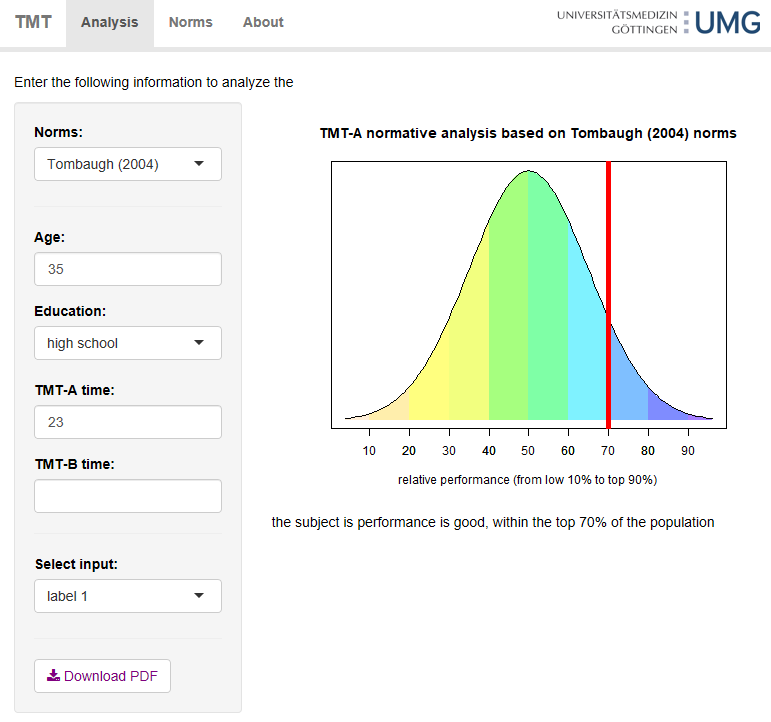
\includegraphics[width=80mm]{./Resources/app-main.png}
	\caption{The main window of the TMT app \label{overflow}}
\end{figure}

\break

To analyze the TMT score with the app, first the normative data to be used for interpreting the data has to be specified. Next, the jubject's age, level of education, and TMT scores (part A, B, or both) should be specified. The app also allows the user to export a PDF document for the analysis report. 




\bibliography{bibliography}

\end{document}
